\documentclass[aspectratio=169,xcolor=dvipsnames]{beamer}
\makeatletter
\def\input@path{{../../common/slides/theme/}{common/slides/theme/}{theme/}}
\makeatother
\usetheme{CleanEasy}
\usepackage[utf8]{inputenc}
\usepackage{lmodern}
\usepackage[T1]{fontenc}
\usepackage{fix-cm}
\usepackage{amsmath}
\usepackage{mathtools}
\usepackage{listings}
\usepackage{xcolor}
\usepackage{hyperref}
\usepackage{graphicx}
\graphicspath{{../../common/slides/assets/}{common/slides/assets/}{./}}
\usepackage{booktabs}
\usepackage{tikz}
\usetikzlibrary{positioning, shapes, arrows, calc, decorations.pathreplacing, arrows.meta, backgrounds, patterns, overlay-beamer-styles, angles, quotes, intersections}
\usepackage{etoolbox}
\usepackage{animate}

\lstset{
  basicstyle=\ttfamily\small,
  keywordstyle=\color{blue},
  commentstyle=\color{green!60!black},
  stringstyle=\color{red},
  showstringspaces=false,
  breaklines=true,
  frame=single,
  rulecolor=\color{black!30},
  backgroundcolor=\color{black!5},
  numbers=left,
  numberstyle=\tiny\color{black!70},
  numbersep=5pt
}

%----------------------------------------------------------------------------------------
%    TITLE PAGE
%----------------------------------------------------------------------------------------

\title[Math Team]{Math Team}
\subtitle{2026--2027 IA\\[0.8em]\textit{``Junior year so chill''}\\[-0.2em]{\scriptsize --Marty Ho}}
\author[IA Math Team]{IA Math Team}
\vspace{-2cm}\date{Aug. 27, 2026}

%----------------------------------------------------------------------------------------

\begin{document}

\begin{frame}[t]
  \titlepage
\end{frame}

%----------------------------------------------------------------------------------------
%    OVERVIEW
%----------------------------------------------------------------------------------------

\begin{frame}[t]{Today}
\vspace{0.35cm}
\begin{enumerate}
    \item Introduction
    \item Teacher Sponsors
    \item Competitions
    \item Resources
    \item Canvas
    \item Jeopardy
\end{enumerate}
\end{frame}

%----------------------------------------------------------------------------------------
%    TEACHER SPONSORS
%----------------------------------------------------------------------------------------

\begin{frame}[t]{Our Teacher Sponsors}
\vspace{0.8cm}
\centering
{\Large Mr. Pomerance}\par\vspace{0.55cm}
{\Large Ms. Pitrak}\par\vspace{0.55cm}
{\Large Mr. Cardwell}
\end{frame}

%----------------------------------------------------------------------------------------
%    COMPETITIONS
%----------------------------------------------------------------------------------------

\begin{frame}[t]{Competitions}
\vspace{0.35cm}
\renewcommand{\arraystretch}{1.45}
\begin{tabular}{p{0.27\textwidth} p{0.63\textwidth}}
\toprule
\textbf{College-hosted} & GT, UGA, KSU, MGA, CSU, Clemson \\
\midrule
\textbf{Nationally-recognized} & AMC 10/12, AIME \\
\midrule
\textbf{Community} & GSMST, Floyd, Westminster, Rockdale \\
\midrule
\textbf{State-wide} & GCTM, GML, GAAPMT \\
\bottomrule
\end{tabular}
\vspace{4em}
\begin{itemize}
    \item And more!
\end{itemize}
\end{frame}

%----------------------------------------------------------------------------------------
%    RESOURCES
%----------------------------------------------------------------------------------------

\begin{frame}[t]{Resources}
\footnotesize
\begin{columns}[T,onlytextwidth]
    \begin{column}{0.34\textwidth}
        \textbf{AMC-Level}\par\vspace{0.35em}
        \href{https://artofproblemsolving.com/alcumus}{Alcumus}\\[0.25em]
        \href{https://artofproblemsolving.com/wiki/index.php/AMC_10_Problems_and_Solutions}{Past AMC 10 Tests}\\[0.25em]
        \href{https://artofproblemsolving.com/wiki/index.php/AMC_12_Problems_and_Solutions}{Past AMC 12 Tests}\\[0.25em]
        \href{https://www.kennesaw.edu/csm/academics/mathematics/ksu-mathematics-competition.php}{Past KSU I Tests}\\[0.25em]
        \href{https://berkeley.mt/archives/}{Past BMT Tests}\\[0.25em]
        \href{https://www.hmmt.org/www/archive/results}{Past HMMT I Tests}
    \end{column}

    \begin{column}{0.31\textwidth}
        \textbf{AIME-Level}\par\vspace{0.35em}
        \href{https://artofproblemsolving.com/wiki/index.php/AIME_Problems_and_Solutions}{Past AIME Tests}\\[0.25em]
        \href{https://www.hmmt.org/www/archive/results}{Past HMMT II Tests}

        \vspace{1.1em}
        \textbf{General}\par\vspace{0.35em}
        \href{https://artofproblemsolving.com/}{AoPS}
    \end{column}

    \begin{column}{0.29\textwidth}
        \textbf{Proofs}\par\vspace{0.35em}
        \href{https://www.kennesaw.edu/csm/academics/mathematics/ksu-mathematics-competition.php}{Past KSU II Tests}\\[0.25em]
        \href{https://math.berkeley.edu/~hutching/teach/proofs.pdf}{Intro to Formal Proofwriting}
    \end{column}
\end{columns}
\vspace{6em}
\begin{itemize}
    \item We'll upload this PDF to our Canvas and you can click on the hyperlinks above.
\end{itemize}
\end{frame}

\begin{frame}[t]{Canvas}
\begin{itemize}
    \item We will try to add all new members into the Canvas as soon as possible.
    \item (Go through Canvas)
    \begin{itemize}
        \item Canvas Announcements will be the primary source of communication for this semester
        \item (Go through all modules)
    \end{itemize}
\end{itemize}
\end{frame}

% The original deck lists Canvas in the agenda, but has no Canvas content slide.

%----------------------------------------------------------------------------------------
%    JEOPARDY
%----------------------------------------------------------------------------------------

{
\usebackgroundtemplate{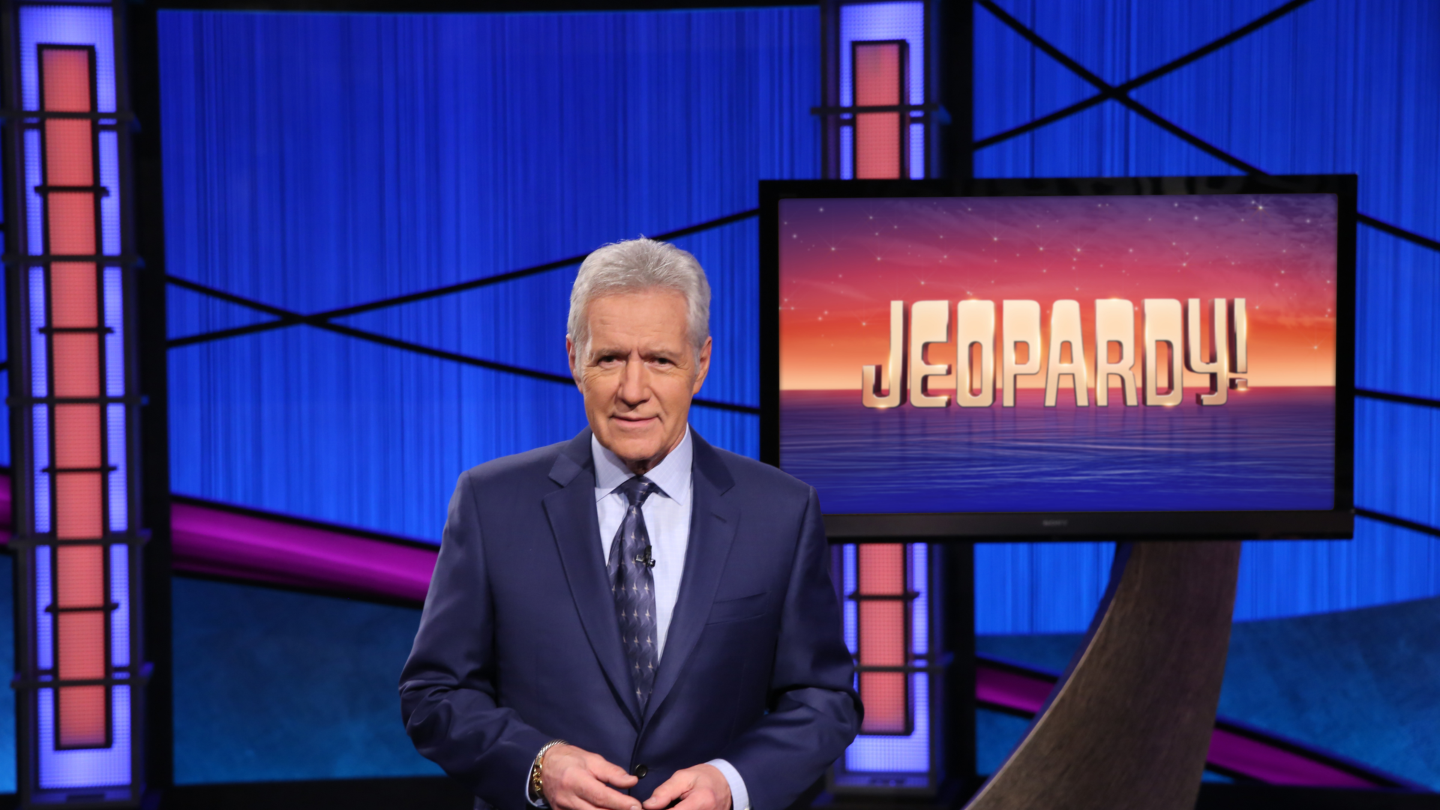
\includegraphics[width=\paperwidth,height=\paperheight]{final-jeopardy.png}}
\begin{frame}[plain]
\end{frame}
}

\end{document}
